\documentclass[12pt,letterpaper]{article}
\usepackage{graphicx,textcomp}
\usepackage{natbib}
\usepackage{setspace}
\usepackage{fullpage}
\usepackage{color}
\usepackage[reqno]{amsmath}
\usepackage{amsthm}
\usepackage{fancyvrb}
\usepackage{amssymb,enumerate}
\usepackage[all]{xy}
\usepackage{endnotes}
\usepackage{lscape}
\newtheorem{com}{Comment}
\usepackage{float}
\usepackage{hyperref}
\newtheorem{lem} {Lemma}
\newtheorem{prop}{Proposition}
\newtheorem{thm}{Theorem}
\newtheorem{defn}{Definition}
\newtheorem{cor}{Corollary}
\newtheorem{obs}{Observation}
\usepackage[compact]{titlesec}
\usepackage{dcolumn}
\usepackage{tikz}
\usetikzlibrary{arrows}
\usepackage{multirow}
\usepackage{xcolor}
\newcolumntype{.}{D{.}{.}{-1}}
\newcolumntype{d}[1]{D{.}{.}{#1}}
\definecolor{light-gray}{gray}{0.65}
\usepackage{url}
\usepackage{listings}
\usepackage{color}

\definecolor{codegreen}{rgb}{0,0.6,0}
\definecolor{codegray}{rgb}{0.5,0.5,0.5}
\definecolor{codepurple}{rgb}{0.58,0,0.82}
\definecolor{backcolour}{rgb}{0.95,0.95,0.92}

\lstdefinestyle{mystyle}{
	backgroundcolor=\color{backcolour},   
	commentstyle=\color{codegreen},
	keywordstyle=\color{magenta},
	numberstyle=\tiny\color{codegray},
	stringstyle=\color{codepurple},
	basicstyle=\footnotesize,
	breakatwhitespace=false,         
	breaklines=true,                 
	captionpos=b,                    
	keepspaces=true,                 
	numbers=left,                    
	numbersep=5pt,                  
	showspaces=false,                
	showstringspaces=false,
	showtabs=false,                  
	tabsize=2
}
\lstset{style=mystyle}
\newcommand{\Sref}[1]{Section~\ref{#1}}
\newtheorem{hyp}{Hypothesis}

\title{Problem Set 3}
\date{Due: November 12, 2026}
\author{William Sarsfield}


\begin{document}
	\maketitle
	\section*{Instructions}
	\begin{itemize}
		\item Please show your work! You may lose points by simply writing in the answer. If the problem requires you to execute commands in \texttt{R}, please include the code you used to get your answers. Please also include the \texttt{.R} file that contains your code. If you are not sure if work needs to be shown for a particular problem, please ask.
	\item Your homework should be submitted electronically on GitHub.
	\item This problem set is due before 23:59 on Thursday November 12, 2026. No late assignments will be accepted.

	\end{itemize}

		\vspace{.25cm}
	
\noindent In this problem set, you will run several regressions and create an add variable plot (see the lecture slides) in \texttt{R} using the \texttt{incumbents\_subset.csv} dataset. Include all of your code.

	\vspace{.5cm}
\section*{Question 1}
\vspace{.25cm}
\noindent We are interested in knowing how the difference in campaign spending between incumbent and challenger affects the incumbent's vote share. 
	\begin{enumerate}
		\item Run a regression where the outcome variable is \texttt{voteshare} and the explanatory variable is \texttt{difflog}.	\vspace{5cm}
		\lstinputlisting[language=R, firstline=36, lastline=37]{PS03_Answers_WS.R}  
			
			\begin{table}[!htbp] \centering 
				\caption{} 
				\label{} 
				\begin{tabular}{@{\extracolsep{5pt}}lc} 
					\\[-1.8ex]\hline 
					\hline \\[-1.8ex] 
					& \multicolumn{1}{c}{\textit{Dependent variable:}} \\ 
					\cline{2-2} 
					\\[-1.8ex] & voteshare \\ 
					\hline \\[-1.8ex] 
					difflog & 0.042$^{***}$ \\ 
					& (0.001) \\ 
					& \\ 
					Constant & 0.579$^{***}$ \\ 
					& (0.002) \\ 
					& \\ 
					\hline \\[-1.8ex] 
					Observations & 3,193 \\ 
					R$^{2}$ & 0.367 \\ 
					Adjusted R$^{2}$ & 0.367 \\ 
					Residual Std. Error & 0.079 (df = 3191) \\ 
					F Statistic & 1,852.791$^{***}$ (df = 1; 3191) \\ 
					\hline 
					\hline \\[-1.8ex] 
					\textit{Note:}  & \multicolumn{1}{r}{$^{*}$p$<$0.1; $^{**}$p$<$0.05; $^{***}$p$<$0.01} \\ 
				\end{tabular} 
			\end{table} 
			
		
			
			
			\textbf{Coefficient:} Every one-unit increase in the logarithmic difference in campaign spending is on average associated with a 4.2 percentage points increase in the vote share of the incumbent. Further since the p-value was significant to the 0.01 level, the difference in campaign spending is a significant predictor of the vote share the incumbent receives.
		
		
		
			\textbf{Intercept:} Further when there is no difference in the logarithmic difference in campaign spending the incumbents vote share will be on average around 57.9 percentage points.
			
			
			
		\item Make a scatterplot of the two variables and add the regression line. 	\vspace{3cm}
			\lstinputlisting[language=R, firstline=38, lastline=45]{PS03_Answers_WS.R}  
			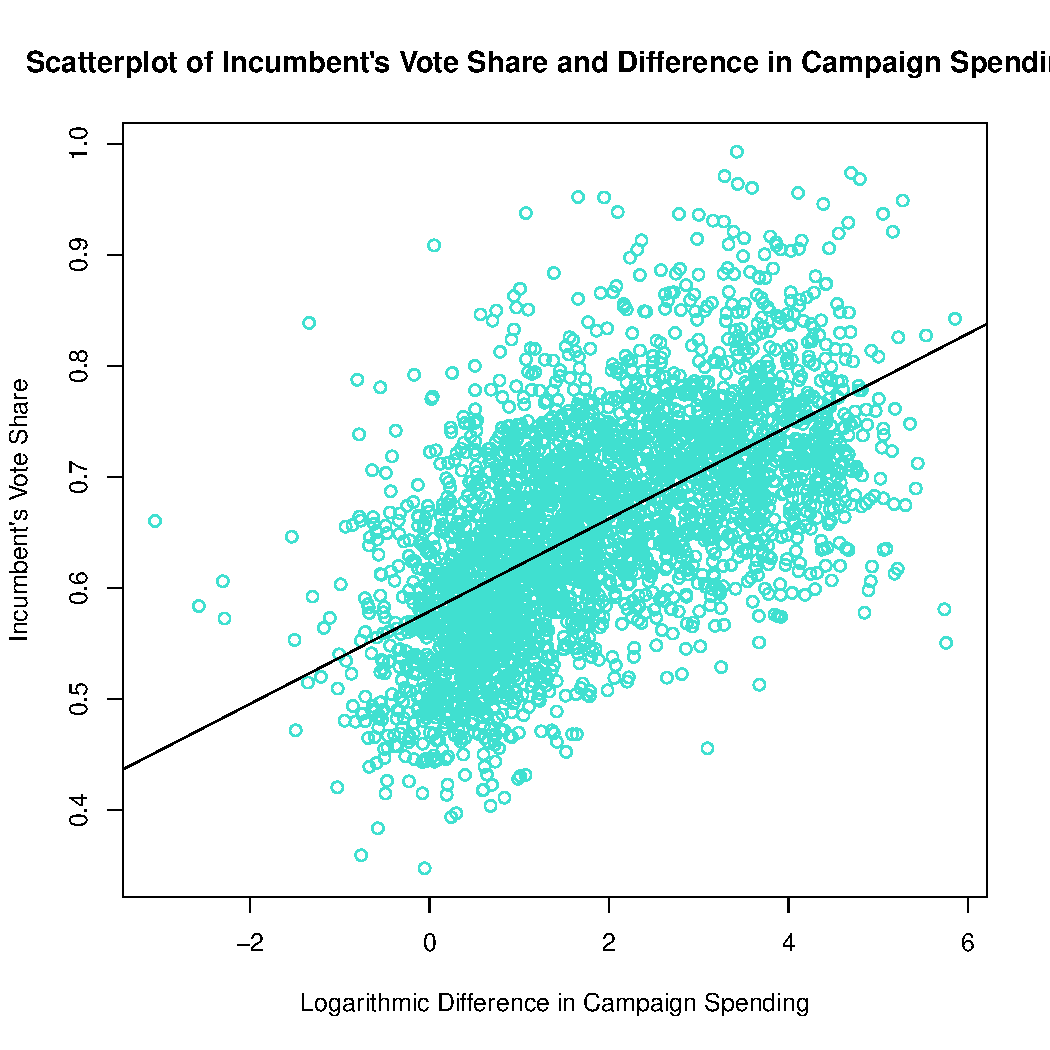
\includegraphics[width=.75\textwidth]{Question1Plot.pdf}
		\item Save the residuals of the model in a separate object.	\vspace{1cm}
		\lstinputlisting[language=R, firstline=46, lastline=46]{PS03_Answers_WS.R}  
		\item Write the prediction equation. \vspace{1cm}
		
		
		$\widehat {Incumbent's Voteshare}$ = .579 + .042 x Difference in Campaign Spending
	\end{enumerate}
	
\newpage

\section*{Question 2}
\noindent We are interested in knowing how the difference between incumbent and challenger's spending and the vote share of the presidential candidate of the incumbent's party are related.	\vspace{.25cm}
	\begin{enumerate}
		\item Run a regression where the outcome variable is \texttt{presvote} and the explanatory variable is \texttt{difflog}.	\vspace{1cm}
		\lstinputlisting[language=R, firstline=49, lastline=50]{PS03_Answers_WS.R}  
		\begin{table}[!htbp] \centering 
			\caption{} 
			\label{} 
			\begin{tabular}{@{\extracolsep{5pt}}lc} 
				\\[-1.8ex]\hline 
				\hline \\[-1.8ex] 
				& \multicolumn{1}{c}{\textit{Dependent variable:}} \\ 
				\cline{2-2} 
				\\[-1.8ex] & presvote \\ 
				\hline \\[-1.8ex] 
				difflog & 0.024$^{***}$ \\ 
				& (0.001) \\ 
				& \\ 
				Constant & 0.508$^{***}$ \\ 
				& (0.003) \\ 
				& \\ 
				\hline \\[-1.8ex] 
				Observations & 3,193 \\ 
				R$^{2}$ & 0.088 \\ 
				Adjusted R$^{2}$ & 0.088 \\ 
				Residual Std. Error & 0.110 (df = 3191) \\ 
				F Statistic & 307.715$^{***}$ (df = 1; 3191) \\ 
				\hline 
				\hline \\[-1.8ex] 
				\textit{Note:}  & \multicolumn{1}{r}{$^{*}$p$<$0.1; $^{**}$p$<$0.05; $^{***}$p$<$0.01} \\ 
			\end{tabular} 
		\end{table} 
		
	\textbf{Coefficient:} Every one-unit increase in the logarithmic difference in campaign spending on average is associated with an increase of 2.4 percentage points in the vote share of the presidential candidate of the incumbent's party. Further since the p-value was significant to the 0.01 level, the difference in campaign spending is a significant predictor of the vote share of the presidential candidate of the incumbent's party.

	\textbf{Intercept:} Further when there is no difference in the logarithmic difference in campaign spending the vote share of the presidential candidate of the incumbent's party will be on average around 50.8 percentage points. 

		
		\item Make a scatterplot of the two variables and add the regression line. 	
		\lstinputlisting[language=R, firstline=51, lastline=57]{PS03_Answers_WS.R}  
		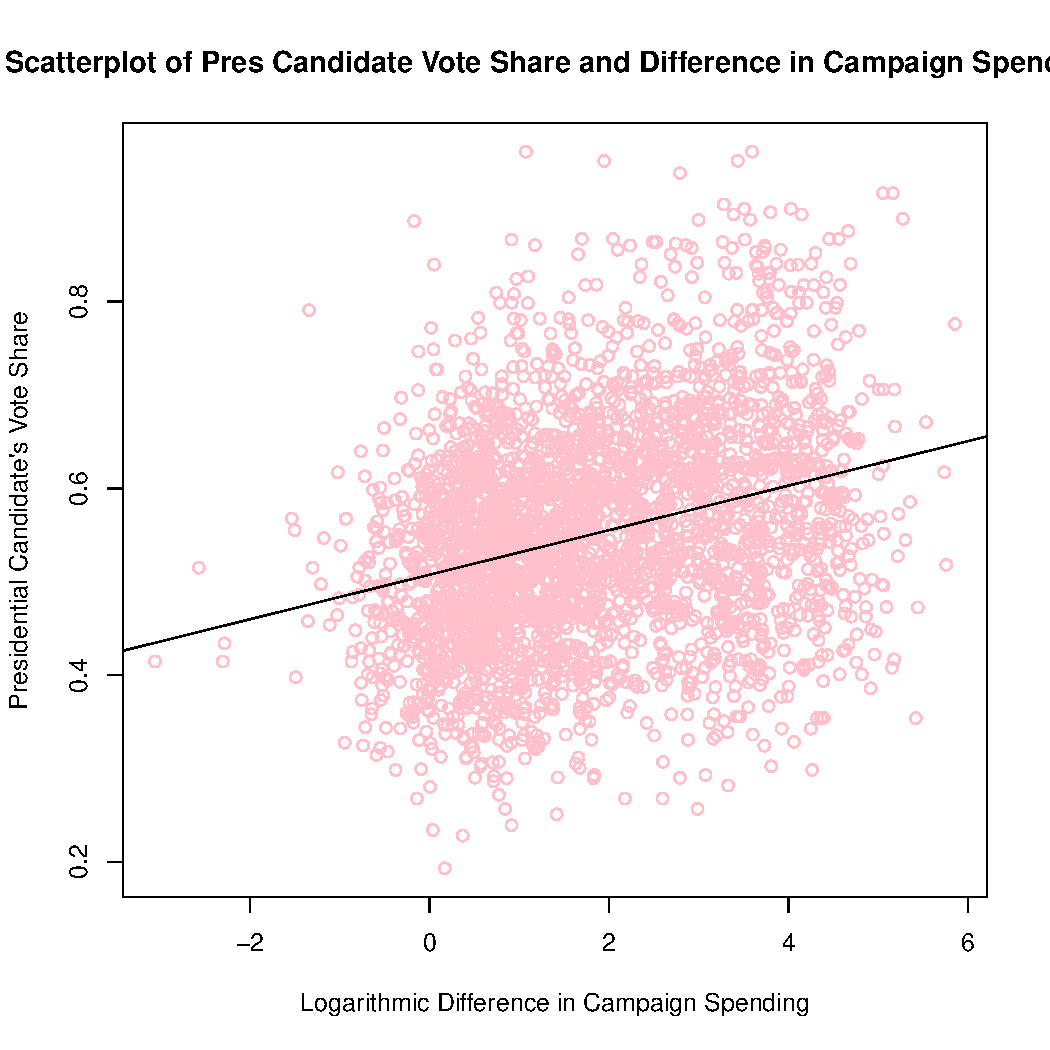
\includegraphics[width=.75\textwidth]{Question2Plot.pdf}
		\item Save the residuals of the model in a separate object.	\vspace{1cm}
			\lstinputlisting[language=R, firstline=58, lastline=58]{PS03_Answers_WS.R}  
		\item Write the prediction equation.
		
		
		$\widehat {Presidential Canidate Vote Share}$ = .508 + .024 x Difference in Campaign Spending
	\end{enumerate}
	
	\newpage	
\section*{Question 3}

\noindent We are interested in knowing how the vote share of the presidential candidate of the incumbent's party is associated with the incumbent's electoral success.
	\vspace{.25cm}
	\begin{enumerate}
		\item Run a regression where the outcome variable is \texttt{voteshare} and the explanatory variable is \texttt{presvote}.
			\vspace{1cm}
			\lstinputlisting[language=R, firstline=61, lastline=62]{PS03_Answers_WS.R}  
			\begin{table}[!htbp] \centering 
				\caption{} 
				\label{} 
				\begin{tabular}{@{\extracolsep{5pt}}lc} 
					\\[-1.8ex]\hline 
					\hline \\[-1.8ex] 
					& \multicolumn{1}{c}{\textit{Dependent variable:}} \\ 
					\cline{2-2} 
					\\[-1.8ex] & voteshare \\ 
					\hline \\[-1.8ex] 
					presvote & 0.388$^{***}$ \\ 
					& (0.013) \\ 
					& \\ 
					Constant & 0.441$^{***}$ \\ 
					& (0.008) \\ 
					& \\ 
					\hline \\[-1.8ex] 
					Observations & 3,193 \\ 
					R$^{2}$ & 0.206 \\ 
					Adjusted R$^{2}$ & 0.206 \\ 
					Residual Std. Error & 0.088 (df = 3191) \\ 
					F Statistic & 826.950$^{***}$ (df = 1; 3191) \\ 
					\hline 
					\hline \\[-1.8ex] 
					\textit{Note:}  & \multicolumn{1}{r}{$^{*}$p$<$0.1; $^{**}$p$<$0.05; $^{***}$p$<$0.01} \\ 
				\end{tabular} 
			\end{table} 
					
					
					\textbf{Coefficient:} Every one-unit increase in the vote share of the presidential candidate of the incumbent's party is associated with an on average increase of 38.8 percentage points in the vote share of the incumbent's party. Further since the p-value is significant to the 0.01 level, the vote share of the presidential candidate of the incumbent's party is a significant predictor of vote share of the incumbent party. 
					
					\textbf{Intercept:} When the vote share of the presidential candidate of the incumbent's party is zero the incumbent party's vote share will be on average around 44.1 percentage points. However, despite being significant to the 0.01 significance level, this value has no meaning in the real world as it is very unlikely verging on improbable that a presidential candidate of the incumbent party would receive 0 percent of the vote share.
					
		\item Make a scatterplot of the two variables and add the regression line. 
			\vspace{1cm}
				\lstinputlisting[language=R, firstline=63, lastline=70]{PS03_Answers_WS.R}  
					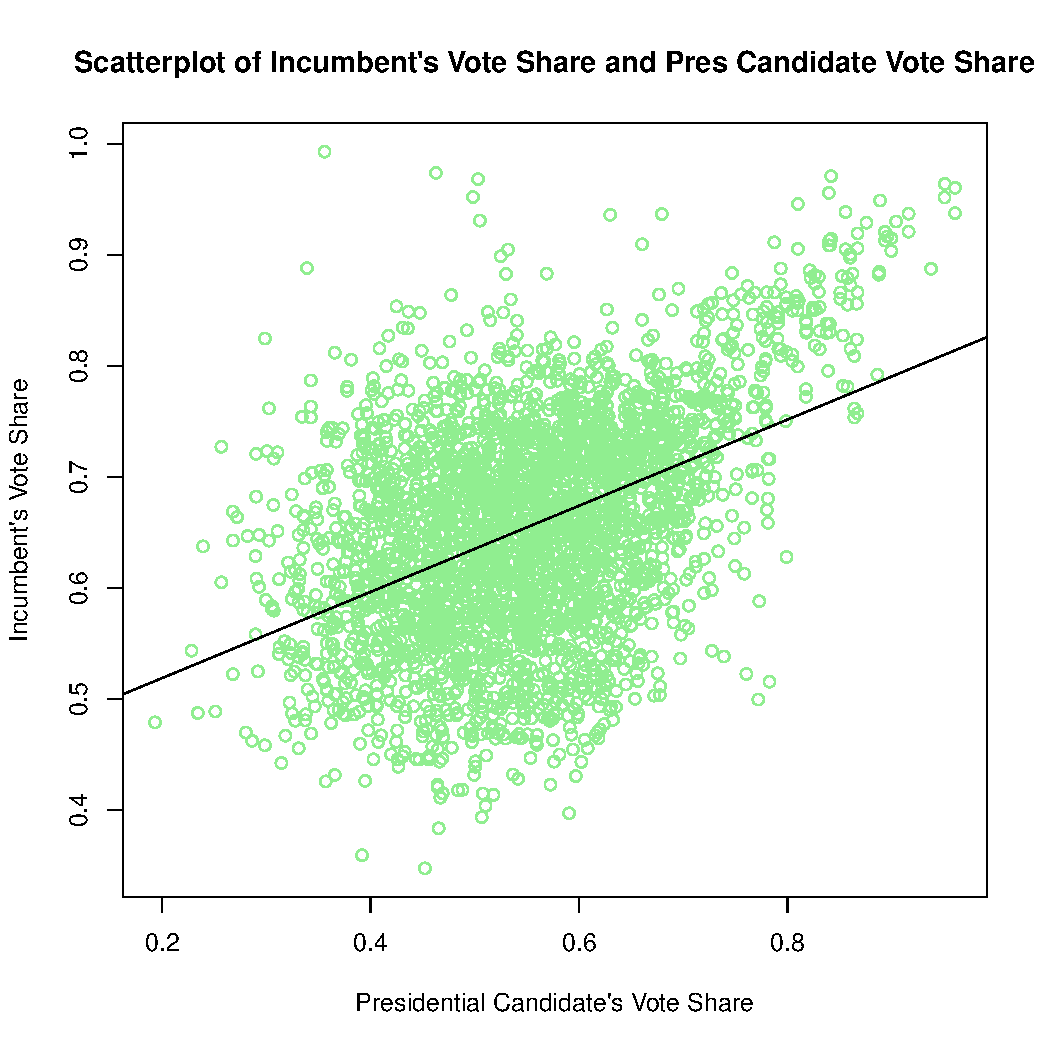
\includegraphics[width=.75\textwidth]{Question3Plot.pdf}
		\item Write the prediction equation.
		\vspace{1cm}
		
			$\widehat {Incumbent's Voteshare}$ = 0.441 + 0.388  x Presidential Candidate Vote Share
	\end{enumerate}
	

\newpage	
\section*{Question 4}
\noindent The residuals from part (a) tell us how much of the variation in \texttt{voteshare} is $not$ explained by the difference in spending between incumbent and challenger. The residuals in part (b) tell us how much of the variation in \texttt{presvote} is $not$ explained by the difference in spending between incumbent and challenger in the district.
	\begin{enumerate}
		\item Run a regression where the outcome variable is the residuals from Question 1 and the explanatory variable is the residuals from Question 2.	\vspace{1cm}
			\lstinputlisting[language=R, firstline=73, lastline=74]{PS03_Answers_WS.R}  
	\begin{table}[!htbp] \centering 
		\caption{} 
		\label{} 
		\begin{tabular}{@{\extracolsep{5pt}}lc} 
			\\[-1.8ex]\hline 
			\hline \\[-1.8ex] 
			& \multicolumn{1}{c}{\textit{Dependent variable:}} \\ 
			\cline{2-2} 
			\\[-1.8ex] & residual1 \\ 
			\hline \\[-1.8ex] 
			residuals2 & 0.257$^{***}$ \\ 
			& (0.012) \\ 
			& \\ 
			Constant & $-$0.000 \\ 
			& (0.001) \\ 
			& \\ 
			\hline \\[-1.8ex] 
			Observations & 3,193 \\ 
			R$^{2}$ & 0.130 \\ 
			Adjusted R$^{2}$ & 0.130 \\ 
			Residual Std. Error & 0.073 (df = 3191) \\ 
			F Statistic & 476.975$^{***}$ (df = 1; 3191) \\ 
			\hline 
			\hline \\[-1.8ex] 
			\textit{Note:}  & \multicolumn{1}{r}{$^{*}$p$<$0.1; $^{**}$p$<$0.05; $^{***}$p$<$0.01} \\ 
		\end{tabular} 
	\end{table} 
			\vspace{1cm}
		\vspace{1cm}
		
	\textbf{Coefficient:} By regressing the residuals, every one-unit increase in the residual from Question 2 (The variation in the vote share of the presidential candidate of the incumbent's party not explained by difference in campaign spending) is associated with a .257 increase in the residual from Question 1 (The variation in the vote share of the incumbent's party not explained by difference in campaign spending). Further since the p-value is significant to the 0.01 level, residual of Question 2 is a significant predictor of the residual from Question 1. 
	
		\textbf{Intercept:} Further, when the residual from Question 2 is zero on average the residual from Question 1 would be zero.
		\item Make a scatterplot of the two residuals and add the regression line. 	\vspace{1cm}
			\lstinputlisting[language=R, firstline=77, lastline=83]{PS03_Answers_WS.R}  
				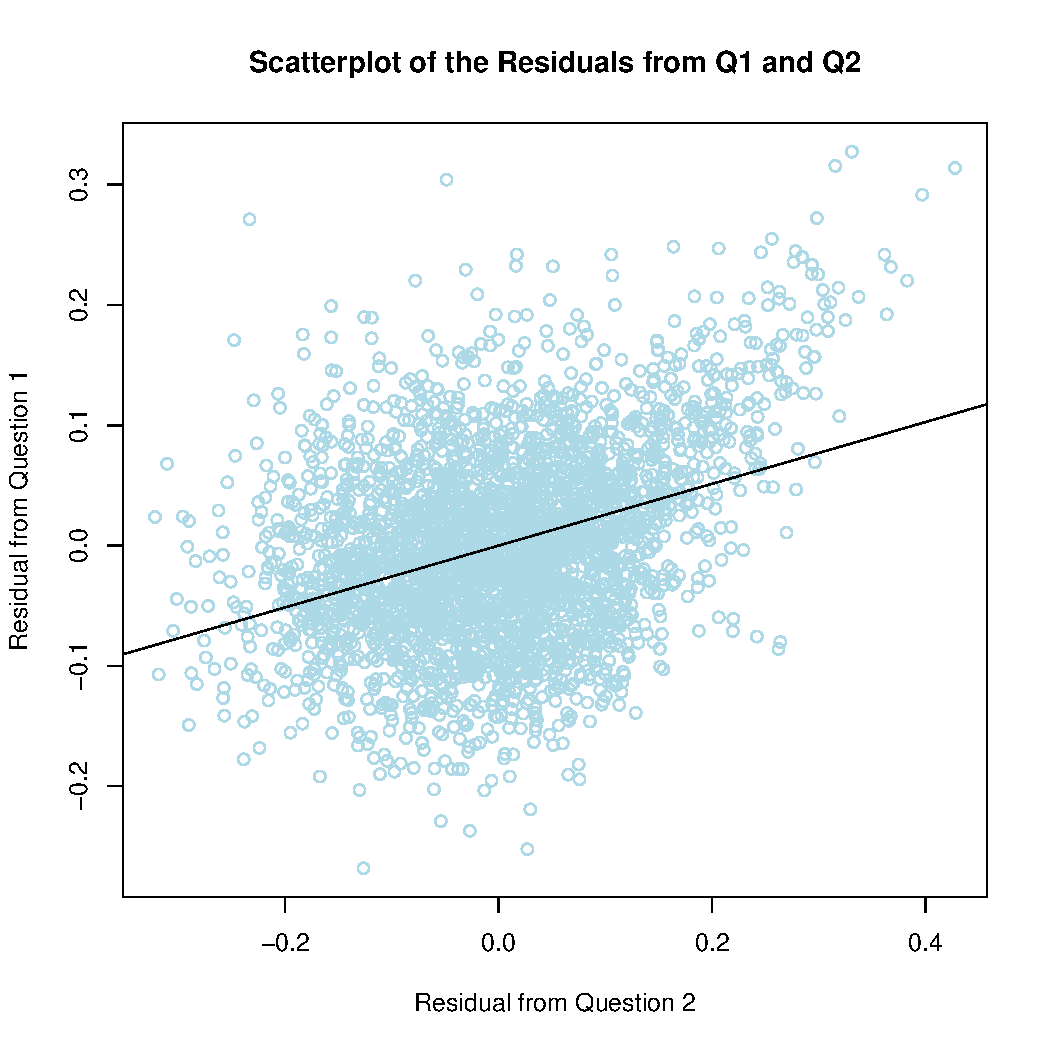
\includegraphics[width=.75\textwidth]{Question4Plot.pdf}
		\item Write the prediction equation.
		
			$\widehat {Residual From Q1}$ =  0 + .257 x Residual From Q2
	\end{enumerate}
	
	\newpage	

\section*{Question 5} 
\noindent What if the incumbent's vote share is affected by both the president's popularity and the difference in spending between incumbent and challenger? 
	\begin{enumerate}
		\item Run a regression where the outcome variable is the incumbent's \texttt{voteshare} and the explanatory variables are \texttt{difflog} and \texttt{presvote}	
		\vspace{1cm}
		/ 
			\lstinputlisting[language=R, firstline=88, lastline=89]{PS03_Answers_WS.R}  
			
			
\begin{table}[!htbp] \centering 
	\caption{} 
	\label{} 
	\begin{tabular}{@{\extracolsep{5pt}}lc} 
		\\[-1.8ex]\hline 
		\hline \\[-1.8ex] 
		& \multicolumn{1}{c}{\textit{Dependent variable:}} \\ 
		\cline{2-2} 
		\\[-1.8ex] & voteshare \\ 
		\hline \\[-1.8ex] 
		difflog & 0.036$^{***}$ \\ 
		& (0.001) \\ 
		& \\ 
		presvote & 0.257$^{***}$ \\ 
		& (0.012) \\ 
		& \\ 
		Constant & 0.449$^{***}$ \\ 
		& (0.006) \\ 
		& \\ 
		\hline \\[-1.8ex] 
		Observations & 3,193 \\ 
		R$^{2}$ & 0.450 \\ 
		Adjusted R$^{2}$ & 0.449 \\ 
		Residual Std. Error & 0.073 (df = 3190) \\ 
		F Statistic & 1,302.947$^{***}$ (df = 2; 3190) \\ 
		\hline 
		\hline \\[-1.8ex] 
		\textit{Note:}  & \multicolumn{1}{r}{$^{*}$p$<$0.1; $^{**}$p$<$0.05; $^{***}$p$<$0.01} \\ 
	\end{tabular} 
\end{table} 
			
			\textbf{Coefficient:} \texttt{DiffLog } Every one-unit increase in the logarithmic difference in campaign spending is associated with an increase of 3.6 percentage points in the vote share of the incumbent party while holding the variation in the \texttt{presvote} variable constant. 
			
			\textbf{Coefficient:} \texttt{Presvote} Every one-unit increase in the vote share of the presidential candidate of the incumbent's party is associated with an increase of 25.7 percentage points (.257 units)  in the vote share of the incumbent's party while holding the variation in the \texttt{difflog} variable constant. 
			
			
		Further since the p-value for both predictors is significant to the 0.01 level, therefore difference in campaign spending is a significant predictor of vote share of incumbent as well as the vote share of the presidential candidate of the incumbent's party is a significant predictor of vote share of the incumbent. 
		
			
			\textbf{Intercept:} Further when both \texttt{difflog} = 0 and \texttt{presvote} = 0  the incumbent party's vote share will be on average around 44.9 percentage points. However as mentioned previously it is very unlikely that a presidential candidate of the incumbent's party will receive zero percent of the vote share therefore the y-intercept has little meaningful interpretation. 
			
			Looking at both the results in Question 3 and Question 5  the difference in campaign spending between the incumbent and challengers is positively correlated with presidential candidate vote share and incumbent vote share. As in Question 3 for every increase of one unit in vote share of the presidential candidate  of the incumbent's party on average vote share of the incumbent party increases by .388 and it decreases to .257 for \textbf{Question 5} therefore signalling that the \texttt{difflog} variable is positively correlated with voteshare and presvote.
			

		
		\item Write the prediction equation.	\vspace{1cm}\\
		$\widehat {Incumbent's Voteshare}$ = 0.449 + 0.036 x Difference in Campaign Spending  + 0.257 x Presidential Candidate Vote Share
		\item What is it in this output that is identical to the output in Question 4? Why do you think this is the case?
		
		
		The Beta of .257 in the residual plot is identical to the Beta of presvote and voteshare in Question 5 while holding the variation in \texttt{difflog} constant. Additionally the Standard Error is also the same. The reason that this is identical is because the residuals from Question 1  told us how much the variation in voteshare was not explained by the difference in spending between incumbent and challenger in a district. Whereas the residual in Question 2 demonstrates the variation in presvote that is not explained by the difference in spending by incumbent and challenger in the district. 
		
		Thus, the residuals presented have removed the effect of \texttt{difflog}, or the difference in campaign spending from both the \texttt{voteshare} and \texttt{presvote} variables. Therefore, by performing a bivariate regression of the residuals in Question 4 and getting a Beta of .257 this regression therefore holds for the variation of \texttt{difflog} constant. The same action is done in the multivariate regression in Question 5. Therefore both regressions effectively do the same action, therefore the variation for \texttt{difflog} is accounted for in both regressions and the coefficient for the Beta and the SE are identical in both Question 4 and 5.
	
		
		
		
		
	
			\end{enumerate}




\end{document}
